\documentclass[11pt,letterpaper]{article}

\usepackage[T1]{fontenc}
\usepackage[utf8]{inputenc}
\usepackage{lmodern}
\usepackage[margin=1in]{geometry}
\usepackage{amsmath,amssymb}
\usepackage{booktabs}
\usepackage{tabularx}
\usepackage{longtable}
\usepackage{graphicx}
\usepackage{float}
\usepackage[font=small,labelfont=bf]{caption}
\usepackage{enumitem}
\usepackage{microtype}
\usepackage[table]{xcolor}
\usepackage[hidelinks]{hyperref}
\usepackage{url}
\usepackage{makecell}

\setlist{itemsep=2pt,topsep=4pt}
\setlength{\parskip}{4pt}
\renewcommand{\arraystretch}{1.15}
\newcommand{\yes}{\textbf{\textcolor{green!45!black}{Yes}}}
\newcommand{\no}{\textcolor{black!45}{--}}
\newcommand{\high}{\cellcolor{red!18}High}
\newcommand{\med}{\cellcolor{orange!22}Medium}
\newcommand{\low}{\cellcolor{green!14}Low}

\title{\vspace{-0.6cm}\rule{\textwidth}{1.4pt}\\[10pt]
\textbf{VEYRA Security Self-Assessment Report: Permission-Tier Implementation and Known-Risk Register}\\[6pt]
\rule{\textwidth}{0.6pt}}

\newcommand{\authorbox}[4]{\begin{tabular}{c}\textbf{#1}\\ #2\\ #3\\ {\small\texttt{#4}}\end{tabular}}
\author{
\begin{tabular}{c@{\hspace{1.4cm}}c}
\authorbox{Athilla Zaidan Zidna Fann}{Informatics Engineering}{Institut Teknologi Bandung}{} &
\authorbox{Jason Edward Salim}{Informatics Engineering}{Institut Teknologi Bandung}{13524034@std.stei.itb.ac.id} \\ \noalign{\vskip 16pt}
\authorbox{Abel Gani}{Information Systems and Technology}{Institut Teknologi Bandung}{18224016@std.stei.itb.ac.id} &
\authorbox{Gregory William Sutjipto}{Information Systems and Technology}{Institut Teknologi Bandung}{18224010@std.stei.itb.ac.id} \\ \noalign{\vskip 16pt}
\multicolumn{2}{c}{\authorbox{Tiffany Viriya Chu}{Information Systems and Technology}{Institut Teknologi Bandung}{18224068@std.stei.itb.ac.id}}
\end{tabular}
}
\date{}

\begin{document}
\maketitle

\begin{abstract}
\noindent This report is the security self-assessment of \textbf{VEYRA}, a Digital Livestock Passport platform whose AI agent prepares insurance applications, premium payments, and claims that execute only after a manager approves them. It documents how the permission tiers are implemented in code and lists the known risks with their current mitigations and planned remediation. The assessment covers the backend (61 endpoints in 19 route modules), the web client, the camera worker interface, the language-model adapter, and the sandbox insurer and payment providers, at commit \texttt{bc7e56c} of the \texttt{main} branch. Four human roles and one machine identity are enforced on every route, with separation of duties between preparing and approving a financial action. Every farm-scoped query is isolated by farm, financial actions are bound to a hashed payload, time-limited, and idempotent, and the language model has no tools and cannot decide or execute anything. These controls are verified by automated tests within the 551-test backend suite. The register lists 16 known risks: three rated \textbf{High}, all of which arise from prototype-grade identity and secrets (static demo tokens, a default service token, demo mode enabled by default) and are scheduled for closure before any pilot handles real farm data.
\end{abstract}

\section{Scope and Method}

\subsection{Scope}

The assessment covers the components in Table~\ref{tab:scope}. All financial providers are sandboxes: no real money moves, no policy is bound, and no claim is filed with a real insurer. The assessment therefore distinguishes risks that are acceptable in the current demonstration from risks that must be closed before a pilot with real farms, insurers, or payments.

\begin{table}[H]
\centering
\caption{Components in scope.}
\label{tab:scope}
\small
\begin{tabularx}{\textwidth}{>{\raggedright\arraybackslash}p{3.6cm}X}
\toprule
Component & Description \\
\midrule
API service & FastAPI, 61 endpoints in 19 route modules, SQLAlchemy~2 persistence, one Docker image \\
Web client & React~19 + TypeScript progressive web app, served by the API on the same origin \\
Camera worker interface & Observation feed and gallery synchronisation authenticated by a service token \\
Perception adapters & Muzzle matcher (ONNX), weight measurement, view selection, tracking \\
Language-model adapter & GPT-6 Luna for explanations, question parsing, and agent phrasing (structured outputs) \\
Sandbox providers & Simulated insurer and payment provider behind provider adapters \\
Storage & Relational database and media files on a local data volume \\
\bottomrule
\end{tabularx}
\end{table}

\subsection{Method}

The assessment combined four activities. (1) A code review of every route's authentication dependency, every role capability, and every farm-scoped query. (2) A review of the financial action lifecycle, the media and upload paths, and the language-model boundary. (3) A lightweight threat model of each trust boundary using the STRIDE categories (spoofing, tampering, repudiation, information disclosure, denial of service, elevation of privilege). (4) Verification against the automated test suite, whose security-relevant tests are listed in Appendix~\ref{app:tests}. Each risk is rated by likelihood and impact on a three-point scale, with the rating given by the higher of the two when either is high.

\section{System and Trust Boundaries}

Figure~\ref{fig:arch} shows the architecture. Table~\ref{tab:boundaries} lists the trust boundaries and the control that authenticates each crossing.

\begin{figure}[H]
\centering
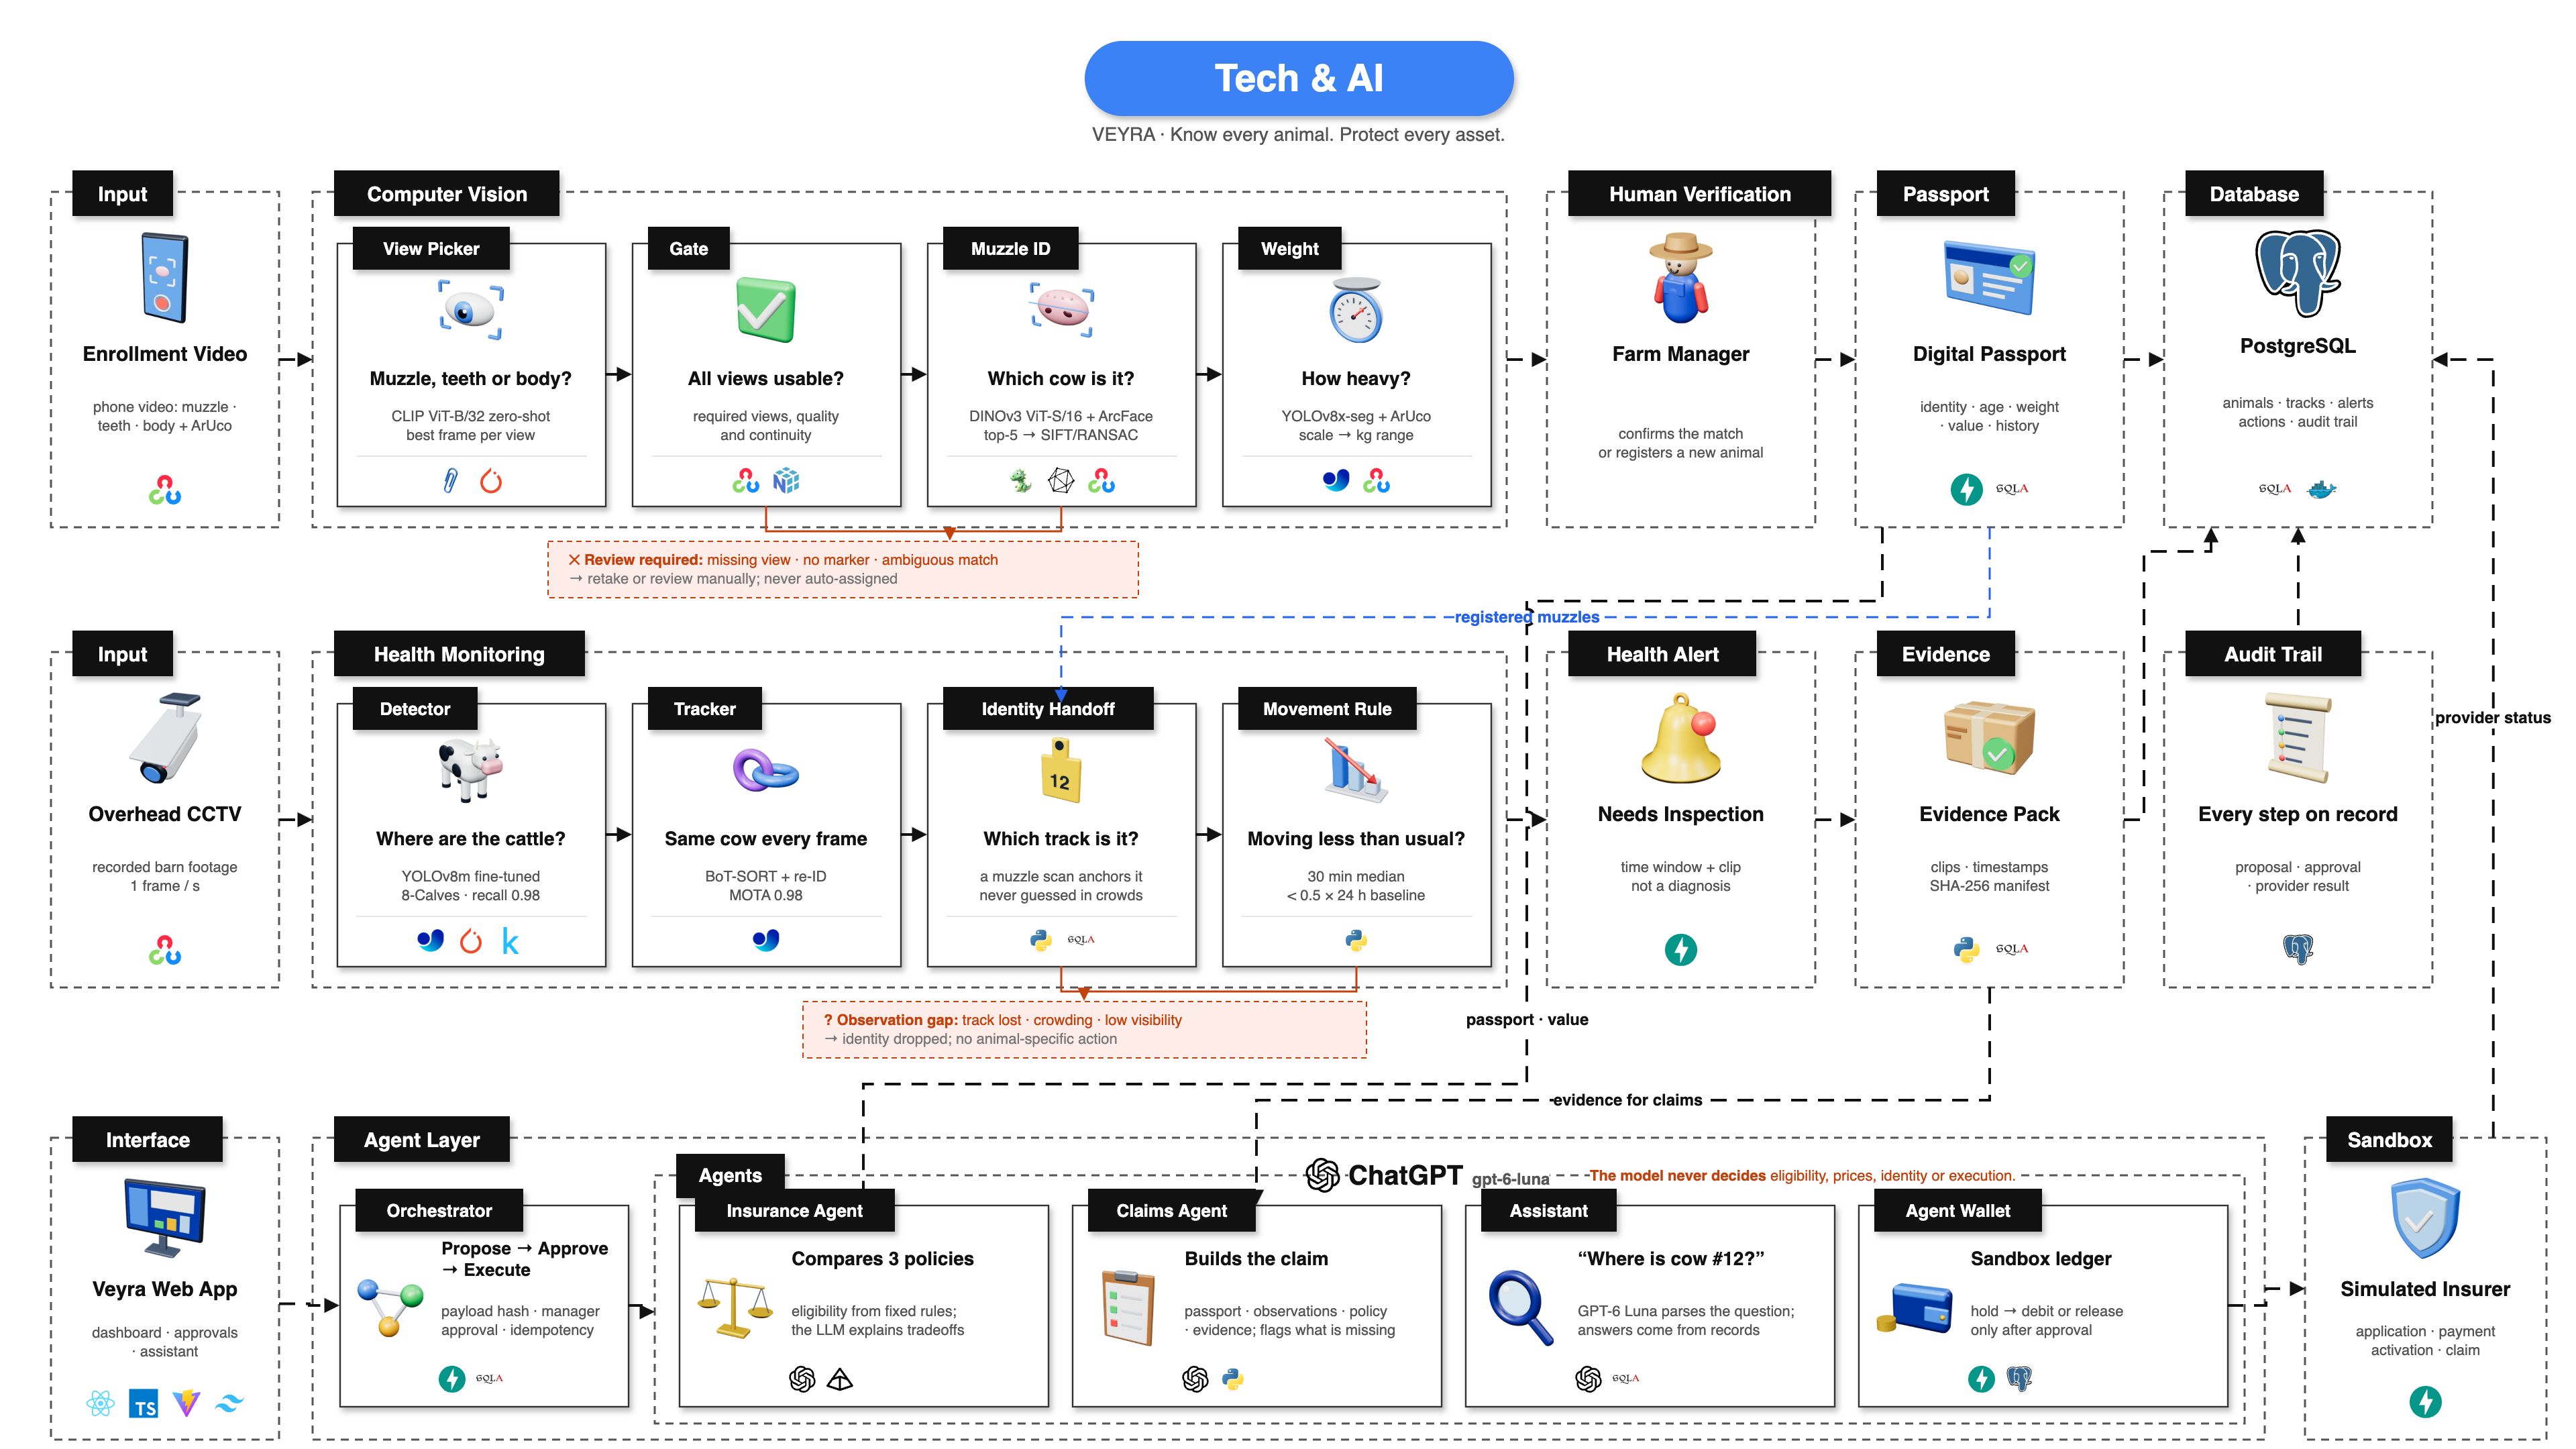
\includegraphics[width=\textwidth]{figures/architecture.png}
\caption{VEYRA architecture. Every human request crosses the API with a bearer token; the camera worker uses a service token; the agent wallet only executes manager-approved payloads.}
\label{fig:arch}
\end{figure}

\begin{table}[H]
\centering
\caption{Trust boundaries and their authentication.}
\label{tab:boundaries}
\small
\begin{tabularx}{\textwidth}{>{\raggedright\arraybackslash}p{3.8cm}>{\raggedright\arraybackslash}p{4.6cm}X}
\toprule
Boundary & Credential & Control \\
\midrule
Browser $\rightarrow$ API & Bearer token per user & Constant-time comparison; role and farm resolved server-side \\
Camera worker $\rightarrow$ API & \texttt{X-Service-Token} & Constant-time comparison; observation feed and gallery acknowledgement only \\
Browser $\rightarrow$ media & Signed URL (\texttt{exp}, \texttt{sig}) & HMAC-SHA256, one-hour expiry, uniform \texttt{NOT\_FOUND} \\
API $\rightarrow$ language model & Provider API key (environment) & Text only, structured outputs, no tools \\
API $\rightarrow$ sandbox providers & In-process adapter & Idempotency key per execution; provider record reconciles retries \\
API $\rightarrow$ storage & Process filesystem & Data volume outside the image; media addressed by id, never by path \\
\bottomrule
\end{tabularx}
\end{table}

\section{Permission-Tier Implementation}

\subsection{Authentication}

A person presents \texttt{Authorization: Bearer <token>}. The API looks the token up in its own short read session, so authentication never holds a write lock, and compares it with \texttt{hmac.compare\_digest} to avoid timing side channels (\texttt{domain/auth.py}). The result is an immutable \texttt{Principal} carrying the user id, farm id, role, and name; the client never supplies its own role or farm. The camera worker presents \texttt{X-Service-Token}, compared the same way, and receives a \texttt{ServicePrincipal} that holds no farm and no human role. A missing or invalid credential always returns the same \texttt{UNAUTHENTICATED} error envelope, and an empty configured service token is rejected rather than treated as a match.

\subsection{Role Tiers}

Roles are declared once as capability tuples, so each route reads as a rule (Table~\ref{tab:tiers}).

\begin{table}[H]
\centering
\caption{Permission tiers and their capability sets.}
\label{tab:tiers}
\small
\begin{tabularx}{\textwidth}{>{\raggedright\arraybackslash}p{2.6cm}>{\raggedright\arraybackslash}p{3.4cm}X}
\toprule
Tier & Capability sets & Authority \\
\midrule
1 · Manager & \texttt{APPROVERS}, \texttt{ENROLLERS}, \texttt{ALERT\_REVIEWERS} & The only role that approves, declines, executes, or reconciles a financial action; confirms claim declarations; publishes the camera gallery; resets the demo \\
2 · Operator & \texttt{ENROLLERS}, \texttt{ALERT\_REVIEWERS} & Enrolls animals, uploads media, confirms valuations, prepares actions, drafts claims, reviews tracks and alerts; cannot approve \\
3 · Veterinarian & \texttt{ALERT\_REVIEWERS}, \texttt{FINDING\_AUTHORS} & The only role that adds professional findings to an incident; no payment authority \\
4 · Assessor & Read only & Reads sandbox submissions; cannot change any record \\
Machine · Service worker & Service token & Posts camera observations and acknowledges gallery versions; no human capability \\
AI agent & None (no principal) & Prepares actions inside a manager's or operator's session; never approves or executes \\
\bottomrule
\end{tabularx}
\end{table}

\subsection{Permission Matrix}

Table~\ref{tab:matrix} maps endpoint groups to tiers, as implemented by the route dependencies (\texttt{require\_roles}, \texttt{service\_principal}, \texttt{service\_or\_roles}).

\begin{table}[H]
\centering
\caption{Permission matrix (M = manager, O = operator, V = veterinarian, A = assessor, S = service worker).}
\label{tab:matrix}
\footnotesize
\setlength{\tabcolsep}{4pt}
\begin{tabularx}{\textwidth}{>{\raggedright\arraybackslash}Xccccc}
\toprule
Operation (endpoint group) & M & O & V & A & S \\
\midrule
Read herd, passports, policies, alerts, claims, audit, wallet & \yes & \yes & \yes & \yes & \no \\
Ask the assistant & \yes & \yes & \yes & \yes & \no \\
Create, upload, process, confirm, retry enrollments & \yes & \yes & \no & \no & \no \\
Confirm valuations; request insurance recommendations & \yes & \yes & \no & \no & \no \\
Propose, revise, cancel agent actions; converse with the agent & \yes & \yes & \no & \no & \no \\
\textbf{Approve or decline, execute, reconcile agent actions} & \yes & \no & \no & \no & \no \\
Record incidents, draft claims, run claim identity checks & \yes & \yes & \no & \no & \no \\
Update a claim (declaration) & \yes & \no & \no & \no & \no \\
Add professional findings & \no & \no & \yes & \no & \no \\
Review alerts & \yes & \yes & \yes & \no & \no \\
Assign tracks; start demo replays & \yes & \yes & \no & \no & \no \\
Policy activation check; publish camera gallery & \yes & \no & \no & \no & \no \\
Post camera observations; acknowledge gallery & \no & \no & \no & \no & \yes \\
Read a camera gallery & \yes & \no & \no & \no & \yes \\
Reset the demo (demo farm and demo mode only); change sandbox settings & \yes & \no & \no & \no & \no \\
\bottomrule
\end{tabularx}
\end{table}

Three routes take no bearer token by design: \texttt{GET /health}, \texttt{GET /media/\{id\}} (the HMAC signature is the credential), and \texttt{GET /demo/footage/\{name\}}, which streams only three named, AI-generated demonstration clips that contain no farm data and exists only in demo mode.

\subsection{Tenant Isolation}

Every farm-scoped query filters on \texttt{Principal.farm\_id}. A record of another farm is reported as \texttt{NOT\_FOUND}, never as forbidden, so a caller cannot even learn that it exists. The same rule protects the camera pipeline: a muzzle match against an animal of another farm is recorded as \texttt{candidate\_not\_registered}, so a camera never learns that another farm's animal exists. The demo reset additionally requires a manager of the demo farm, so a manager of another farm cannot reset it.

\subsection{Approval-Bound Financial Actions}

Financial integrity rests on the action lifecycle rather than on the user interface:
\begin{itemize}
\item \textbf{Server-built payloads.} The server builds every payload from current records; the client never supplies an amount, recipient, or term.
\item \textbf{Hash binding.} The payload is fixed by $h = \mathrm{SHA256}(\mathrm{canonical\_json}(\text{payload}))$, and an approval must name the exact hash and version that the manager reviewed.
\item \textbf{Separation of duties.} Only a manager approves, and an operator cannot approve an action even when the operator prepared it.
\item \textbf{Expiry and staleness.} An action expires 30 minutes after it is proposed. Before execution the payload is rebuilt from current records; any change to amount, recipient, terms, animal, or evidence cancels the approval as \texttt{approval\_stale}.
\item \textbf{Idempotent execution.} Execution requires an \texttt{Idempotency-Key}; a key reused for another action, or a new key after success, is rejected as a duplicate. Execution runs as three short transactions with a balance hold, so a timeout keeps the hold and a retry reconciles from the provider's record instead of paying twice.
\item \textbf{Non-repudiation.} The agent's proposal, the manager's decision, and the provider's result are three separate audit events tied to one animal. The audit module only inserts events; it exposes no update or delete path.
\end{itemize}

\subsection{AI Agent Containment}

The language model is confined to language. It has no tools and cannot call the API. Every call uses a typed output schema, and every system prompt ends with an instruction to treat the farm user's text as data and never as instructions. Eligibility, prices, identity, and execution are computed by deterministic code; explanations are checked against the inputs, and items for products that were not supplied or terms references that do not exist are dropped before display. The in-app agent prepares actions but never approves them: its action-review card points to a pending action that only a manager can stamp. If the model is unavailable, refuses, or returns unparseable output, a deterministic template states the same facts and is labelled as such.

\subsection{Media and Upload Controls}

\begin{itemize}
\item \textbf{Signed downloads.} Media URLs carry \texttt{exp} and $\mathit{sig} = \mathrm{HMAC\text{-}SHA256}(\mathit{secret}, \texttt{id:exp})$ with a one-hour lifetime. A bad, tampered, or expired signature, an unknown id, and a missing file all return the same \texttt{NOT\_FOUND}, so ids cannot be probed.
\item \textbf{Safe serving.} Responses set \texttt{X-Content-Type-Options: nosniff}, and documents download as attachments instead of rendering in the application's origin.
\item \textbf{Type allow-lists.} Videos, photos, and documents are accepted only from explicit content-type lists; documents are also checked by magic bytes (PDF, JPEG, PNG), so a renamed file is refused.
\item \textbf{Size caps.} 200\,MiB for enrollment videos, 50\,MiB for claim identity scans, and 10\,MiB for documents, enforced while streaming and refused early from the \texttt{Content-Length} header.
\item \textbf{Integrity.} Every stored file is hashed with SHA-256 as it is written, and evidence manifests cite those hashes.
\end{itemize}

\subsection{Identity Assurance Controls}

Because the platform's value depends on the right animal being insured and claimed, identity is treated as a security control. A muzzle match must exceed five geometrically verified points with crop quality of at least 0.6, a crowded scan zone identifies nobody, and an identity released by the continuity policy is never re-attached automatically. Every death claim requires a fresh muzzle scan that is matched against the claimed animal \emph{and} every other confirmed animal of the farm; a mismatch names the other animal and blocks submission, and a newer check after approval makes the approved submission stale.

\section{Known-Risk Register}

Table~\ref{tab:risks} lists the known risks. Ratings describe exposure in a pilot or production deployment; in the current sandbox demonstration no real funds or real farm records are at stake.

{\footnotesize
\setlength{\tabcolsep}{3.5pt}
\begin{longtable}{>{\raggedright\arraybackslash}p{0.7cm}>{\raggedright\arraybackslash}p{3.3cm}c>{\raggedright\arraybackslash}p{4.3cm}>{\raggedright\arraybackslash}p{4.6cm}}
\caption{Known-risk register.}\label{tab:risks}\\
\toprule
ID & Risk & Rating & Current mitigation & Planned remediation \\
\midrule
\endfirsthead
\toprule
ID & Risk & Rating & Current mitigation & Planned remediation \\
\midrule
\endhead
\bottomrule
\endfoot
R1 & Static, guessable demo bearer tokens; no login, session expiry, or MFA; tokens stored in plain text & \high & Tokens compared in constant time; tokens resolve role and farm server-side; demo-only users & OIDC/SSO login, short-lived signed sessions, hashed tokens, MFA for managers \\
R2 & Default service token (\texttt{demo-worker-token}) when \texttt{VEYRA\_SERVICE\_TOKEN} is unset & \high & Service tier limited to observations and gallery acknowledgement & Refuse to start outside demo mode without a secret; per-camera credentials or mTLS \\
R3 & Demo mode on by default: reset, sandbox switches, replays, and public footage route exposed & \high & Reset requires a manager of the demo farm; footage route serves three fixed clips without farm data & Default \texttt{VEYRA\_DEMO\_MODE=false} in production builds; deployment check \\
R4 & Farm-wide read access for every role, including the assessor (wallet, audit, all passports) & \med & Reads stay scoped to the user's farm; all writes are role-gated & Per-role read scopes; assessor limited to submitted claims and their evidence \\
R5 & No rate limiting or brute-force protection on authentication, uploads, and assistant queries & \med & Upload size caps; uniform errors reveal nothing to enumerate & Gateway rate limits per token and IP; per-farm quotas on model calls \\
R6 & Transport security delegated: the container serves HTTP on port 8000; no CSP or frame headers & \med & Same-origin web app; \texttt{nosniff} on media; documents as attachments & TLS termination with HSTS; Content-Security-Policy, \texttt{X-Frame-Options}, Referrer-Policy \\
R7 & Data at rest unencrypted on a local volume (database and media), no backup policy & \med & Data volume outside the image; media addressed by id; SHA-256 per file & Managed PostgreSQL with encryption at rest, backups, and point-in-time recovery; encrypted object storage \\
R8 & Audit trail append-only in application code but not tamper-evident in storage & \med & No update or delete path in the audit module; separate proposal, decision, and result events & Hash-chained audit events and write-once storage for the audit log \\
R9 & Presentation attack on the muzzle biometric (printed or replayed muzzle of another animal) & \med & Continuous guided video; human confirmation; claim-time re-scan against every confirmed animal & Liveness and presentation-attack detection on the enrollment and claim scans \\
R10 & Wrong identity association on CCTV in barns unlike the tuning footage & \low & \texttt{handoff\_v2} releases doubtful identities (zero wrong identities on real footage); crowded scans identify nobody & Revalidate on each farm's footage before enabling alerts; cattle-specific re-identification \\
R11 & Prompt injection through farm text or documents; farm data sent to a third-party model provider & \med & No tools; typed outputs; grounding check; text treated as data; deterministic fallback & Data-processing agreement, data minimisation (no personal data in prompts), regional or self-hosted model option \\
R12 & Personal data obligations (farmer, staff, and veterinarian names) under Indonesia's Personal Data Protection Law (UU No.~27/2022) & \med & Minimal personal data; role-based access; no sale or sharing & Privacy notice and consent, retention policy, data-subject request process \\
R13 & Availability: background jobs and camera replays run in one API process & \low & Single worker by design; three-step execution survives restarts via reconciliation & Separate job workers and queue; health checks and autoscaling \\
R14 & Uploaded files are not malware-scanned & \low & Type allow-lists, magic bytes, size caps; files never rendered in the app origin & Antivirus scanning in the upload pipeline \\
R15 & Media links keep working until expiry once shared; random per-process media secret if unset & \low & One-hour expiry; HMAC signature; uniform \texttt{NOT\_FOUND} & Shorter lifetimes for documents; require a configured secret and key rotation \\
R16 & Third-party licences and supply chain (Ultralytics AGPL-3.0, DINOv3 licence, CDN-free build) & \low & Locked dependencies (\texttt{uv.lock}, \texttt{pnpm-lock.yaml}); licences recorded in the model cards & Licence review before closed-source distribution; dependency scanning in CI \\
\end{longtable}
}

\section{Remediation Roadmap}

The risks are scheduled against the product roadmap so that each control is in place before the exposure it addresses becomes real.

\begin{table}[H]
\centering
\caption{Remediation plan by phase.}
\label{tab:roadmap}
\small
\begin{tabularx}{\textwidth}{>{\raggedright\arraybackslash}p{4.2cm}>{\raggedright\arraybackslash}p{2.6cm}X}
\toprule
Phase & Risks closed & Exit criterion \\
\midrule
Before a pilot with real farm data & R1, R2, R3, R6 & Real login with MFA for managers, no default secrets, demo mode off, TLS and security headers \\
During the identity and monitoring pilot & R4, R5, R7, R11, R12 & Least-privilege reads, rate limits, encrypted managed database with backups, data-processing agreement, privacy notice \\
Before connecting a real insurer or payment provider & R8, R9, R14, R15 & Tamper-evident audit, presentation-attack detection, malware scanning, external penetration test \\
At scale & R10, R13, R16 & Per-farm revalidation of tracking, separate job workers, dependency and licence scanning in CI \\
\bottomrule
\end{tabularx}
\end{table}

\section{Conclusion}

VEYRA's core security property, that no money moves and no claim is submitted without a manager approving exactly what will happen, is enforced in the backend by role tiers, separation of duties, hash-bound and time-limited approvals, idempotent execution, and an audit trail that separates agent, human, and provider. Tenant isolation, signed media, upload validation, and a language model without tools complete the defence. The highest risks are prototype-grade identity and secrets, which are expected for a sandbox demonstration and are the first items on the remediation plan before any real farm, insurer, or payment provider is connected.

\appendix
\section{Appendix A: Security Tests}
\label{app:tests}

The following automated tests from the backend suite verify the controls described in this report.

\begin{table}[H]
\centering
\footnotesize
\begin{tabularx}{\textwidth}{>{\raggedright\arraybackslash}p{4.2cm}X}
\toprule
Control & Tests \\
\midrule
Authentication & \texttt{test\_\allowbreak{}missing\_\allowbreak{}token\_\allowbreak{}is\_\allowbreak{}unauthenticated}, \texttt{test\_\allowbreak{}bad\_\allowbreak{}token\_\allowbreak{}is\_\allowbreak{}unauthenticated}, \texttt{test\_\allowbreak{}read\_\allowbreak{}routes\_\allowbreak{}require\_\allowbreak{}a\_\allowbreak{}token}, \texttt{test\_\allowbreak{}service\_\allowbreak{}token\_\allowbreak{}accepted}, \texttt{test\_\allowbreak{}service\_\allowbreak{}token\_\allowbreak{}rejected}, \texttt{test\_\allowbreak{}authenticate\_\allowbreak{}service\_\allowbreak{}rejects\_\allowbreak{}empty\_\allowbreak{}configured\_\allowbreak{}token}, \texttt{test\_\allowbreak{}observation\_\allowbreak{}feed\_\allowbreak{}requires\_\allowbreak{}the\_\allowbreak{}service\_\allowbreak{}token}, \texttt{test\_\allowbreak{}gallery\_\allowbreak{}needs\_\allowbreak{}the\_\allowbreak{}service\_\allowbreak{}token\_\allowbreak{}or\_\allowbreak{}a\_\allowbreak{}manager} \\
Role tiers and separation of duties & \texttt{test\_\allowbreak{}operator\_\allowbreak{}cannot\_\allowbreak{}approve}, \texttt{test\_\allowbreak{}operator\_\allowbreak{}cannot\_\allowbreak{}approve\_\allowbreak{}what\_\allowbreak{}the\_\allowbreak{}agent\_\allowbreak{}prepared}, \texttt{test\_\allowbreak{}operator\_\allowbreak{}decision\_\allowbreak{}is\_\allowbreak{}forbidden\_\allowbreak{}even\_\allowbreak{}when\_\allowbreak{}operator\_\allowbreak{}proposed}, \texttt{test\_\allowbreak{}operator\_\allowbreak{}cannot\_\allowbreak{}run\_\allowbreak{}the\_\allowbreak{}activation\_\allowbreak{}check}, \texttt{test\_\allowbreak{}operator\_\allowbreak{}cannot\_\allowbreak{}reset}, \texttt{test\_\allowbreak{}route\_\allowbreak{}rejects\_\allowbreak{}vet\_\allowbreak{}and\_\allowbreak{}other\_\allowbreak{}farm} \\
Tenant isolation & \texttt{test\_\allowbreak{}cross\_\allowbreak{}farm\_\allowbreak{}action\_\allowbreak{}access\_\allowbreak{}is\_\allowbreak{}not\_\allowbreak{}found}, \texttt{test\_\allowbreak{}other\_\allowbreak{}farm\_\allowbreak{}cannot\_\allowbreak{}see\_\allowbreak{}passport}, \texttt{test\_\allowbreak{}other\_\allowbreak{}farm\_\allowbreak{}animal\_\allowbreak{}is\_\allowbreak{}not\_\allowbreak{}found}, \texttt{test\_\allowbreak{}other\_\allowbreak{}farm\_\allowbreak{}cannot\_\allowbreak{}see\_\allowbreak{}or\_\allowbreak{}review\_\allowbreak{}the\_\allowbreak{}alert}, \texttt{test\_\allowbreak{}other\_\allowbreak{}farm\_\allowbreak{}sees\_\allowbreak{}only\_\allowbreak{}its\_\allowbreak{}own\_\allowbreak{}herd\_\allowbreak{}and\_\allowbreak{}audit}, \texttt{test\_\allowbreak{}other\_\allowbreak{}farm\_\allowbreak{}events\_\allowbreak{}are\_\allowbreak{}not\_\allowbreak{}in\_\allowbreak{}the\_\allowbreak{}passbook}, \texttt{test\_\allowbreak{}other\_\allowbreak{}farms\_\allowbreak{}see\_\allowbreak{}no\_\allowbreak{}scan\_\allowbreak{}zone\_\allowbreak{}of\_\allowbreak{}ours}, \texttt{test\_\allowbreak{}other\_\allowbreak{}farm\_\allowbreak{}manager\_\allowbreak{}cannot\_\allowbreak{}reset\_\allowbreak{}the\_\allowbreak{}demo}, \texttt{test\_\allowbreak{}unregistered\_\allowbreak{}or\_\allowbreak{}other\_\allowbreak{}farm\_\allowbreak{}candidate\_\allowbreak{}leaves\_\allowbreak{}the\_\allowbreak{}track\_\allowbreak{}unassigned} \\
Financial integrity & \texttt{test\_\allowbreak{}charge\_\allowbreak{}is\_\allowbreak{}idempotent\_\allowbreak{}per\_\allowbreak{}key}, \texttt{test\_\allowbreak{}duplicate\_\allowbreak{}execution\_\allowbreak{}is\_\allowbreak{}rejected}, \texttt{test\_\allowbreak{}key\_\allowbreak{}reused\_\allowbreak{}for\_\allowbreak{}another\_\allowbreak{}action\_\allowbreak{}is\_\allowbreak{}duplicate}, \texttt{test\_\allowbreak{}new\_\allowbreak{}key\_\allowbreak{}after\_\allowbreak{}success\_\allowbreak{}is\_\allowbreak{}duplicate}, \texttt{test\_\allowbreak{}declined\_\allowbreak{}action\_\allowbreak{}cannot\_\allowbreak{}execute}, \texttt{test\_\allowbreak{}execution\_\allowbreak{}blocked\_\allowbreak{}after\_\allowbreak{}expired\_\allowbreak{}approval}, \texttt{test\_\allowbreak{}execution\_\allowbreak{}blocked\_\allowbreak{}after\_\allowbreak{}stale\_\allowbreak{}approval}, \texttt{test\_\allowbreak{}new\_\allowbreak{}valuation\_\allowbreak{}after\_\allowbreak{}approving\_\allowbreak{}payment\_\allowbreak{}is\_\allowbreak{}stale}, \texttt{test\_\allowbreak{}payment\_\allowbreak{}decline\_\allowbreak{}fails\_\allowbreak{}and\_\allowbreak{}releases\_\allowbreak{}hold} \\
Media and uploads & \texttt{test\_\allowbreak{}tampered\_\allowbreak{}signature\_\allowbreak{}is\_\allowbreak{}not\_\allowbreak{}found}, \texttt{test\_\allowbreak{}expired\_\allowbreak{}signature\_\allowbreak{}is\_\allowbreak{}not\_\allowbreak{}found}, \texttt{test\_\allowbreak{}unknown\_\allowbreak{}media\_\allowbreak{}is\_\allowbreak{}not\_\allowbreak{}found}, \texttt{test\_\allowbreak{}verify\_\allowbreak{}signature\_\allowbreak{}rejects\_\allowbreak{}empty\_\allowbreak{}and\_\allowbreak{}expired}, \texttt{test\_\allowbreak{}store\_\allowbreak{}rejects\_\allowbreak{}content\_\allowbreak{}type\_\allowbreak{}outside\_\allowbreak{}allow\_\allowbreak{}list}, \texttt{test\_\allowbreak{}oversize\_\allowbreak{}upload\_\allowbreak{}is\_\allowbreak{}refused\_\allowbreak{}from\_\allowbreak{}its\_\allowbreak{}content\_\allowbreak{}length} \\
Identity assurance & \texttt{test\_\allowbreak{}crowded\_\allowbreak{}scan\_\allowbreak{}identifies\_\allowbreak{}nobody\_\allowbreak{}and\_\allowbreak{}raises\_\allowbreak{}no\_\allowbreak{}animal\_\allowbreak{}alert}, \texttt{test\_\allowbreak{}an\_\allowbreak{}empty\_\allowbreak{}zone\_\allowbreak{}identifies\_\allowbreak{}nobody}, \texttt{test\_\allowbreak{}sample\_\allowbreak{}mismatch\_\allowbreak{}blocks\_\allowbreak{}submission\_\allowbreak{}with\_\allowbreak{}the\_\allowbreak{}reason}, \texttt{test\_\allowbreak{}later\_\allowbreak{}mismatch\_\allowbreak{}makes\_\allowbreak{}an\_\allowbreak{}approved\_\allowbreak{}submission\_\allowbreak{}stale}, \texttt{test\_\allowbreak{}no\_\allowbreak{}enrolled\_\allowbreak{}image\_\allowbreak{}is\_\allowbreak{}uncertain\_\allowbreak{}not\_\allowbreak{}a\_\allowbreak{}mismatch} \\
\bottomrule
\end{tabularx}
\end{table}

\section{Appendix B: Deployment Hardening Checklist}

\begin{table}[H]
\centering
\small
\begin{tabularx}{\textwidth}{>{\raggedright\arraybackslash}p{4.6cm}X}
\toprule
Setting & Production value \\
\midrule
\texttt{VEYRA\_DEMO\_MODE} & \texttt{false}: hides reset, replays, sandbox switches, and the footage route \\
\texttt{VEYRA\_SERVICE\_TOKEN} & A long random secret per deployment, rotated; never the default \\
\texttt{VEYRA\_MEDIA\_SECRET} & A long random secret, so signed links survive restarts and keys can be rotated \\
\texttt{VEYRA\_DATABASE\_URL} & A managed, encrypted database with backups \\
Model provider key & Stored in the platform's secret manager, never in the image or repository \\
Reverse proxy & TLS, HSTS, security headers, request size limits, and rate limits \\
\bottomrule
\end{tabularx}
\end{table}

\section{Appendix C: Product Links}

\noindent GitHub repository: \url{https://github.com/ShibainuID/Veyra}

\end{document}
